\documentclass{beamer}
\mode<presentation>
{
  \usetheme{myulm}
  \setbeamercovered{transparent}
  \setbeamertemplate{navigation symbols}{} % no navigation bar
  \setbeamersize{sidebar width left=1.17cm}
}

\usepackage[ngerman]{babel}
\usepackage[utf8]{inputenc}
\usepackage{amsmath,amssymb,amsfonts}
\usepackage{times}
\usepackage{graphicx}
\usepackage{fancyvrb}
\usepackage{array}
\usepackage{colortbl}
\usepackage{nameref}
\usepackage[export]{adjustbox}

\hyphenation{Sil-ben-trenn-ung}

% Anfang der Titelfolie
% Anpassung von: Titel, Untertitel, Autor, Datum und Institut

\title{\LaTeX - praktische Anwendung in wissenschaftlichen Arbeiten}
\subtitle{Hausarbeit Präsentation}
\author{Maximilian Hauser}
\newcommand{\presdatum}{\today} % alternativ zu \today: Eingabe eines festen Datums
\institute
{Medieninformatik B.Sc.\\}
%Ende der Titelfolie

% Anfang der Kopfzeile der Folien
% Anpassung von: Zwischentitel, Leitthema oder Name
% Das Datum wird oben geändert: unter \presdatum{}!

\newcommand{\zwischentitel}{\insertsection}
\newcommand{\leitthema}{\LaTeX - praktische Anwendung in wissenschaftlichen Arbeiten}
% Ende der Kopfzeile

% Anfang der Folien
\begin{document}
\hspace*{-1.49cm}
\frame[plain]{\titlepage}

% Das Inhaltsverzeichnis
\section*{Inhaltsverzeichnis}
\hspace*{-0.7cm}
\begin{frame}
  \frametitle{Inhaltsverzeichnis}
  \tableofcontents
\end{frame}


% 1. Folie
\section{Meine Lieblingsstadt}
\begin{frame}
  \begin{overlayarea}{\textwidth}{6cm}
  \frametitle{Stuttgart}
\vspace{-0.5cm}
\begin{columns}
  \begin{column}{0.7\textwidth}
    \uncover<2->{ \textbf{Basisdaten:}}
     \begin{itemize}
      \item<3-> \textbf{Bundesland:}	Baden-Württemberg
      \item<4-> \textbf{Regierungsbezirk:}	Stuttgart
      \item<5-> \textbf{Einwohner:}	626.275
      \item<6-> \textbf{Kfz-Kennzeichen:}	S
     \end{itemize}
  \end{column}
  \begin{column}{0.3\textwidth}  %%<--- here
      \begin{center}
        \includegraphics<2->[width=\textwidth]{rohmaterial-bilder/stuttgart.jpeg}
       \end{center}
  \end{column}
  \end{columns}
 \vspace{1cm}\uncover<7->{\textbf{Warum mag ich diese Stadt so sehr?}} \\
 \uncover<8->{Stuttgart gehört zu den nächstgrößeren Städten nach Ulm im Umkreis. Dort zuhause ist ebenfalls mein Lieblignsfußballverein der VfB Stuttgart. Ebenfalls hat Stuttgart eine sehr schöne Innenstadt, in welcher man sehr viele verschieden Dinge unternehmen kann}
\end{overlayarea}
\end{frame}

% 3. Folie
\section{Meine Lieblingsland}
\begin{frame}
  \begin{overlayarea}{\textwidth}{6cm}
  \frametitle{Schweden}
\vspace{-0.5cm}
\begin{columns}
  \begin{column}{0.7\textwidth}
    \uncover<2->{ \textbf{Basisdaten:}}
     \begin{itemize}
      \item<3-> \textbf{Sprache:}	Schwedisch
      \item<4-> \textbf{Hauptstadt:}	Stockholm
      \item<5-> \textbf{Fläche:}	447.435km²
      \item<6-> \textbf{Einwohnerzahl:}	10.452.326
     \end{itemize}
  \end{column}
  \begin{column}{0.3\textwidth}  %%<--- here
      \begin{center}
        \includegraphics<2->[width=\textwidth]{rohmaterial-bilder/schweden.jpg}
       \end{center}
  \end{column}
  \end{columns}
 \vspace{1cm}\uncover<7->{\textbf{Warum mag ich dieses Land so sehr?}} \\
 \uncover<8->{In meinen Augen ist Schweden das perfekte Land, wenn man gerne Schnee und Wald um sich hat. Vor allem wenn man ein Schneemensch ist, sind die Winter dort besonders schön und ebenfalls sind Städte wie Stockholm und Göteborg sehr schöne Orte zu besuchen}
\end{overlayarea}
\end{frame}

\section{Meine Lieblingsstadt \& mein Lieblingland}
\begin{frame}
\begin{figure}[ht]
  \begin{minipage}[b]{0.45\linewidth}
      \centering
      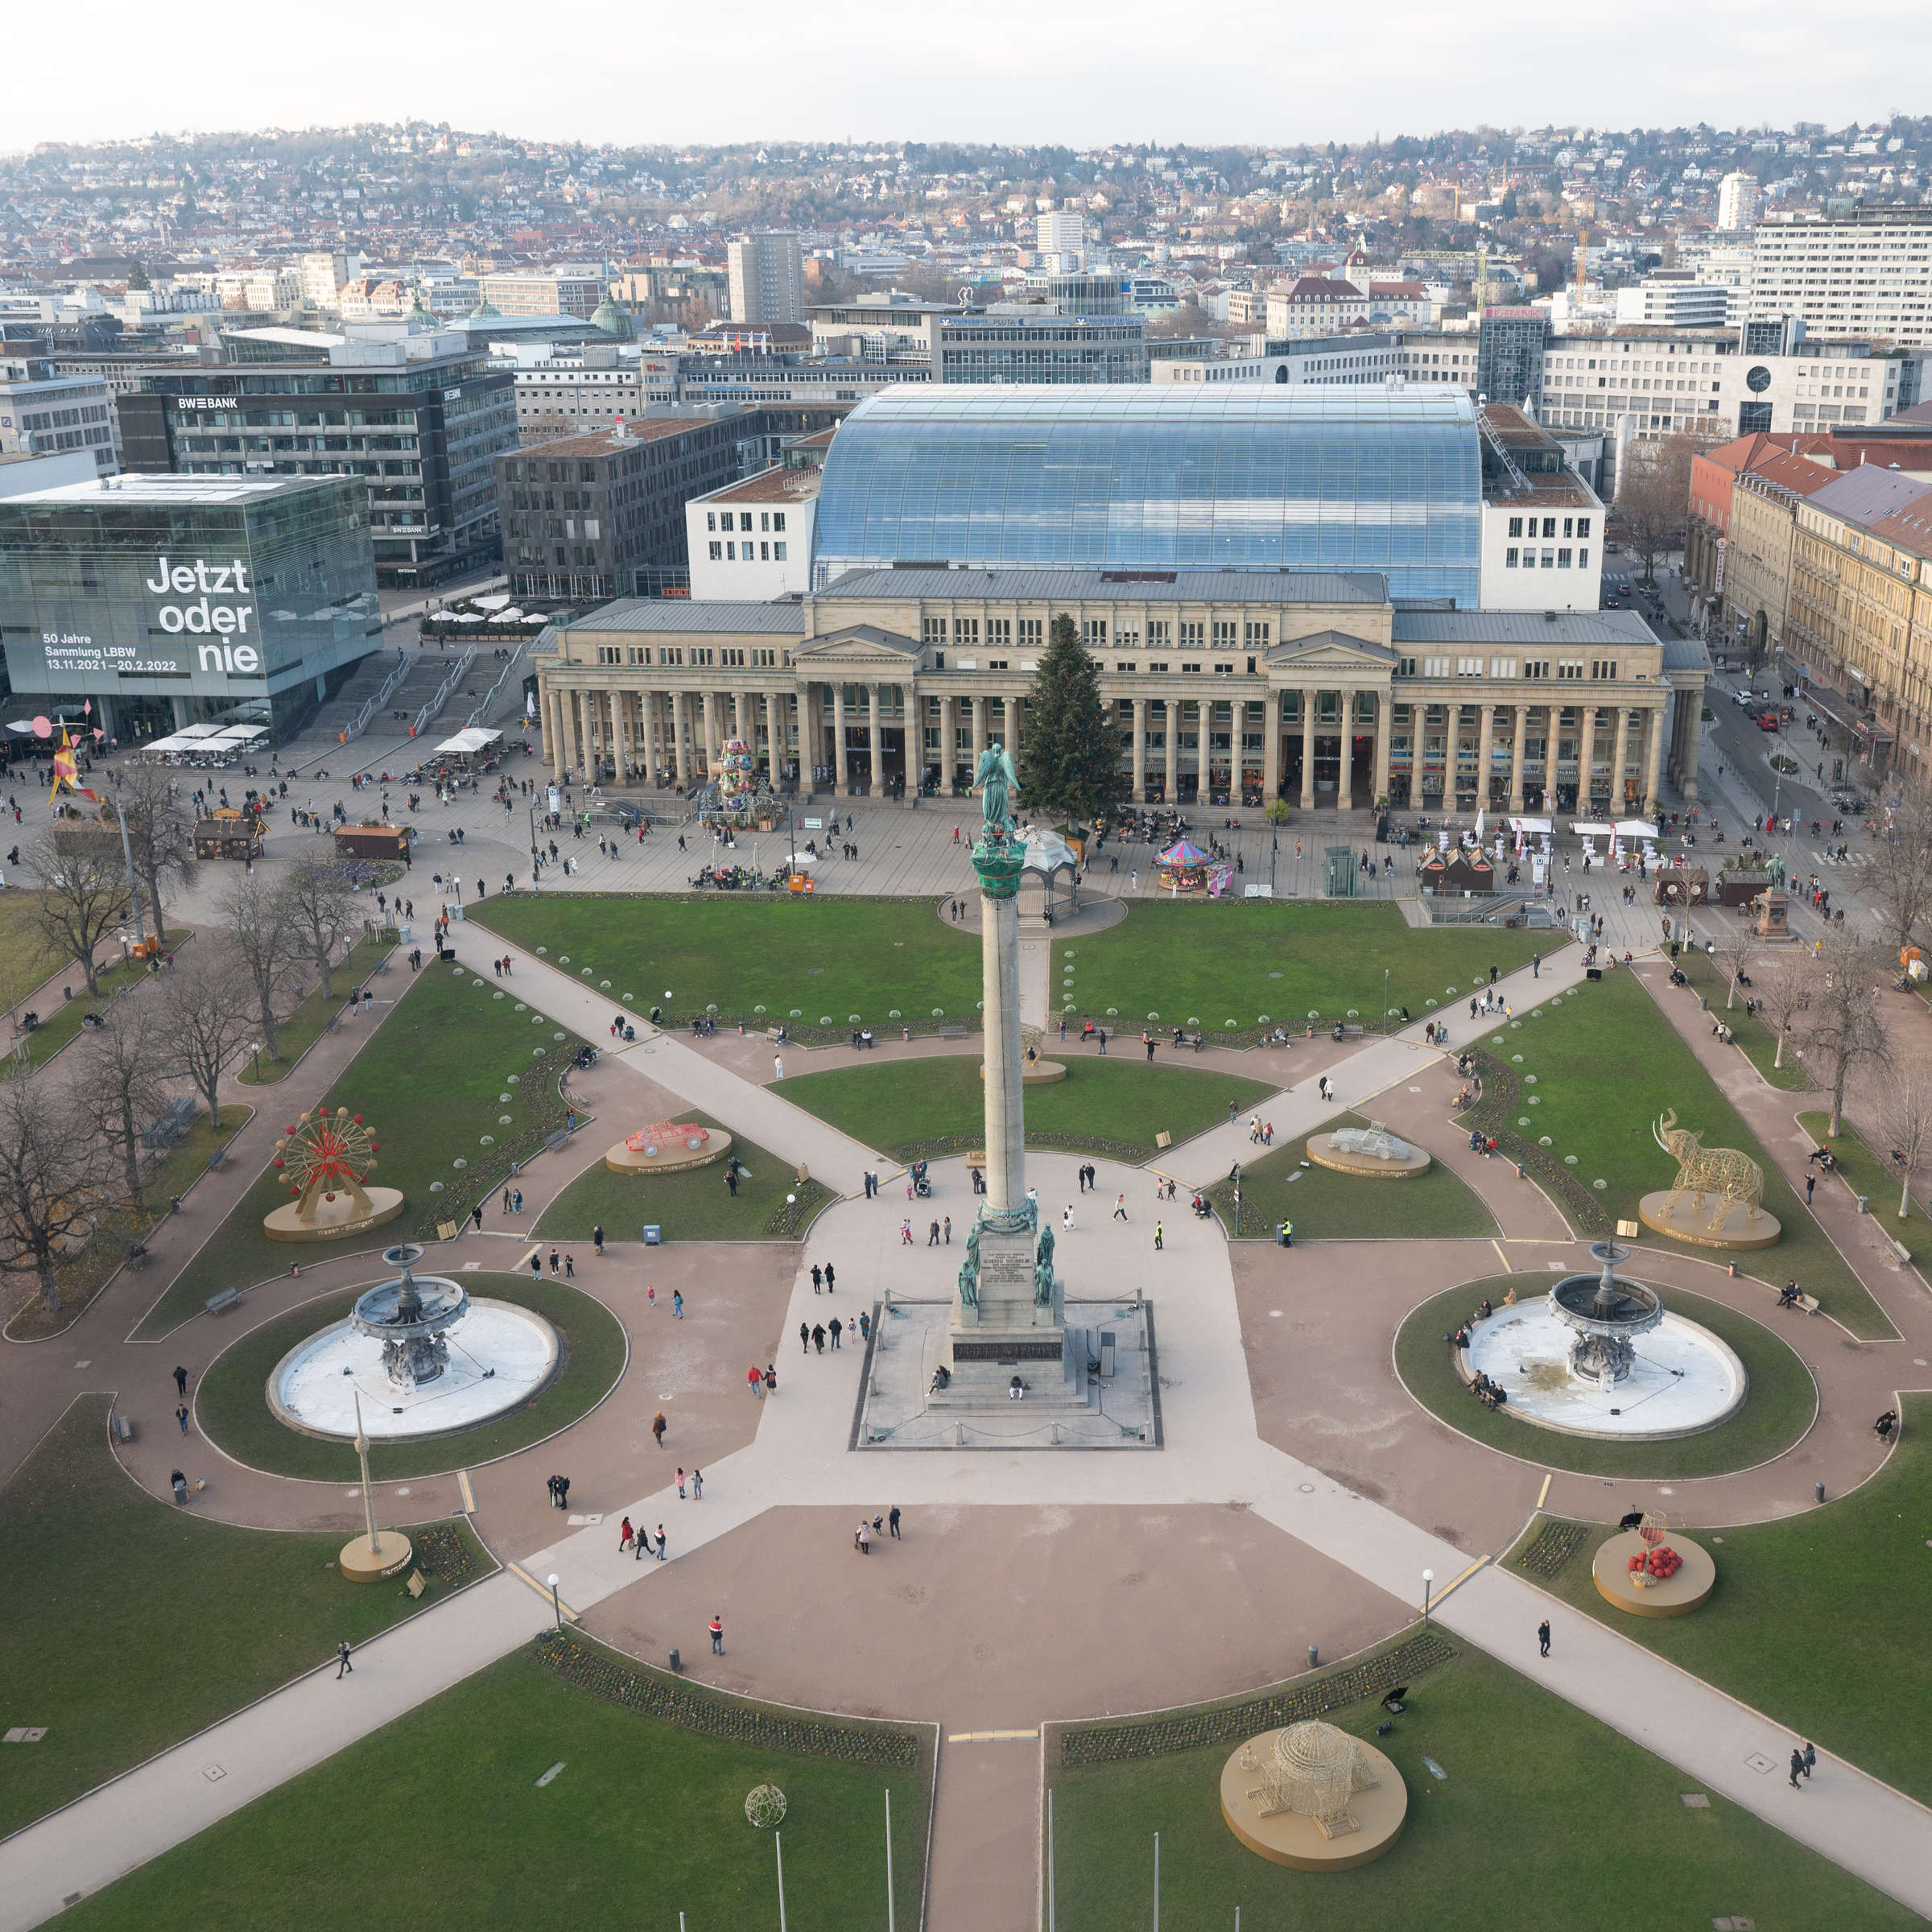
\includegraphics[width=\textwidth, valign=t]{rohmaterial-bilder/Stuttgart.jpeg}
      \caption{Stuttgart}
  \end{minipage}
  \hspace{0.5cm}
  \begin{minipage}[b]{0.45\linewidth}
      \centering
      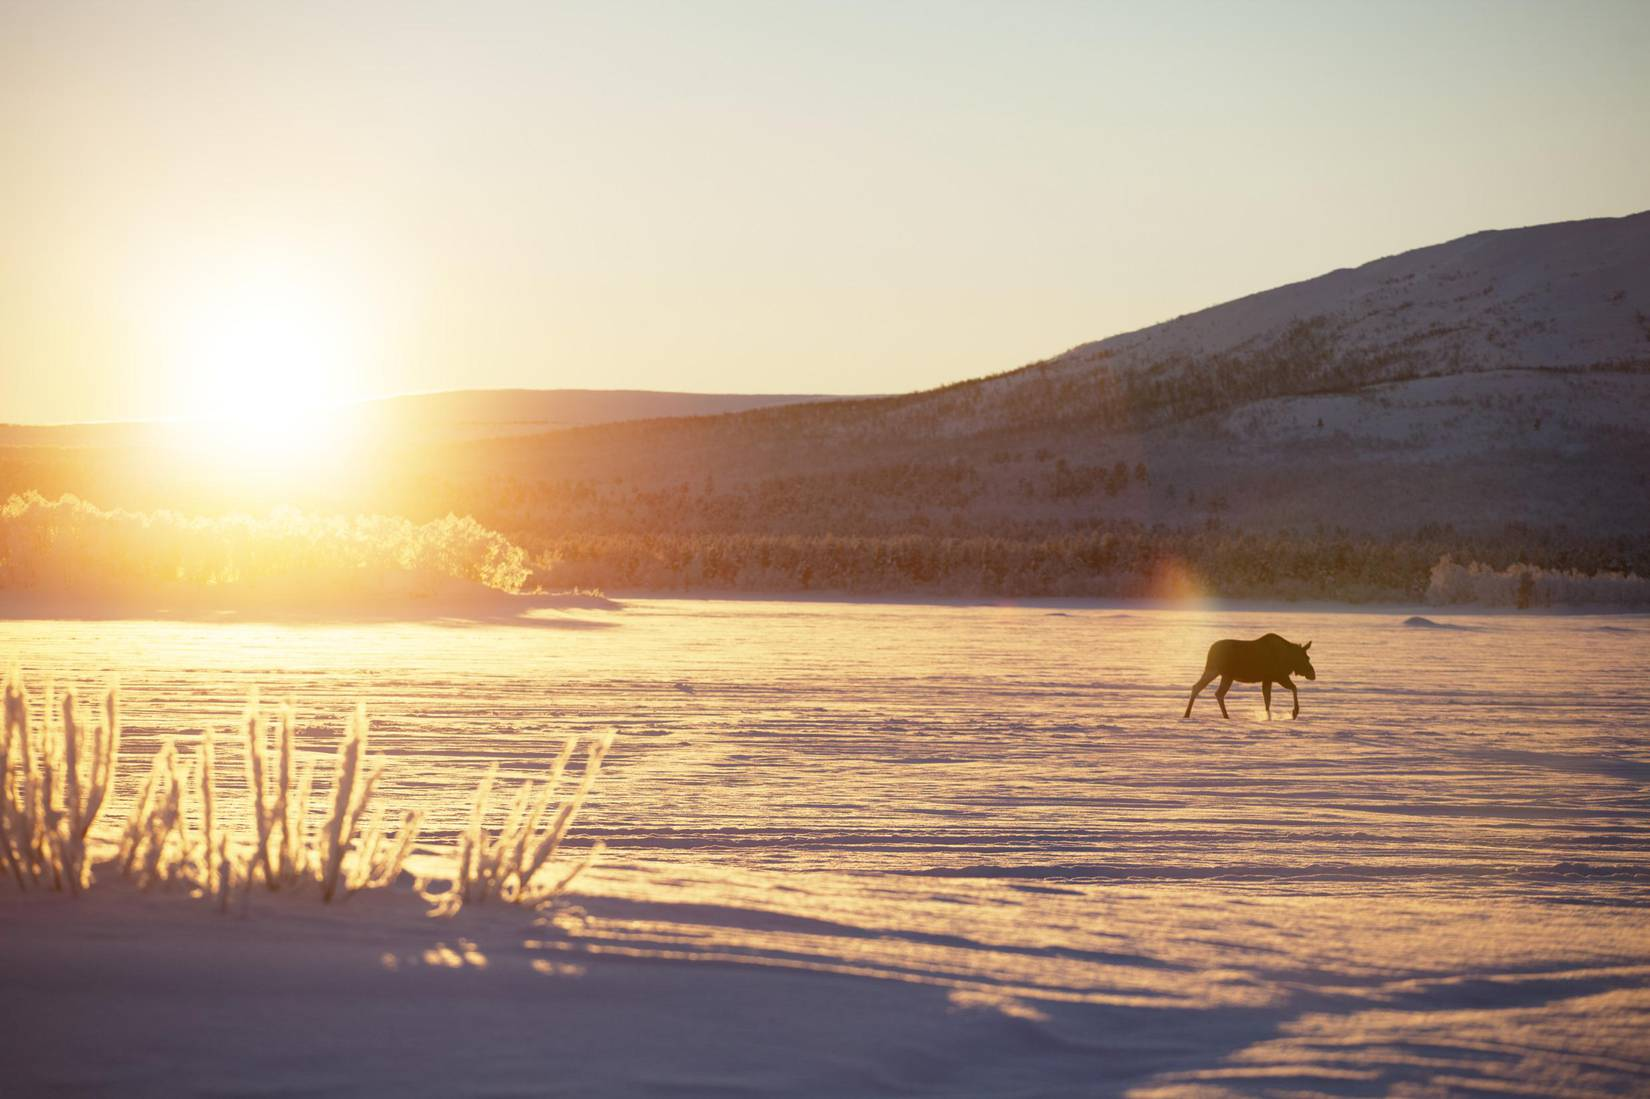
\includegraphics[width=\textwidth, valign=t]{rohmaterial-bilder/schweden.jpg}
      \caption{Schweden}
  \end{minipage}
\end{figure}
\end{frame}
   
% 4. Folie
\section{Quellen}
\begin{frame}
  \frametitle{\insertsection}
 \vspace{-2cm}
 \hspace{-0.8cm}
 \\
  \textbf{Daten:} \\
  \begin{itemize}
    \item \href{https://de.wikipedia.org/wiki/Stuttgart}{Daten Stuttgart}
    \item \href{https://de.wikipedia.org/wiki/Schweden}{Daten Schweden}
  \end{itemize}
    \textbf{Bilder:}
  \begin{itemize}
    \item \href{https://www.echo24.de/bilder/2020/04/22/13753996/schlossplatz-stuttgart-2kZQ5m3gqvec.jpg}{Bild Stuttgart}
    \item \href{https://d3aux7tjp119y2.cloudfront.net/images/ima120004-CMSTemplate_7y0VwYj.width-1650.jpg}{Bild Schweden}
  \end{itemize}

  \end{frame}

% 5. Folie
\section{Über mich}
\begin{frame}
  \frametitle{\insertshortauthor}
\vspace{-0.5cm}
\begin{columns}
  \begin{column}{0.6\textwidth}
     \begin{itemize}
      \item 20 Jahre alt
      \item kommme aus Ehingen
      \item Studiere Medieninformatik im 5. Semester
      \item Neben dem Studium als Foto-/Videograf tätig
     \end{itemize}
  \end{column}
  \begin{column}{0.4\textwidth}  %%<--- here
      \begin{center}
        \includegraphics[width=\textwidth]{rohmaterial-bilder/About.jpg}
       \end{center}
  \end{column}
  \end{columns}
\end{frame}
%Ende der Folien

\end{document}